\documentclass[twoside]{book}

% Packages required by doxygen
\usepackage{fixltx2e}
\usepackage{calc}
\usepackage{doxygen}
\usepackage{graphicx}
\usepackage[utf8]{inputenc}
\usepackage{makeidx}
\usepackage{multicol}
\usepackage{multirow}
\PassOptionsToPackage{warn}{textcomp}
\usepackage{textcomp}
\usepackage[nointegrals]{wasysym}
\usepackage[table]{xcolor}

% Font selection
\usepackage[T1]{fontenc}
\usepackage{mathptmx}
\usepackage[scaled=.90]{helvet}
\usepackage{courier}
\usepackage{amssymb}
\usepackage{sectsty}
\renewcommand{\familydefault}{\sfdefault}
\allsectionsfont{%
  \fontseries{bc}\selectfont%
  \color{darkgray}%
}
\renewcommand{\DoxyLabelFont}{%
  \fontseries{bc}\selectfont%
  \color{darkgray}%
}
\newcommand{\+}{\discretionary{\mbox{\scriptsize$\hookleftarrow$}}{}{}}

% Page & text layout
\usepackage{geometry}
\geometry{%
  a4paper,%
  top=2.5cm,%
  bottom=2.5cm,%
  left=2.5cm,%
  right=2.5cm%
}
\tolerance=750
\hfuzz=15pt
\hbadness=750
\setlength{\emergencystretch}{15pt}
\setlength{\parindent}{0cm}
\setlength{\parskip}{0.2cm}
\makeatletter
\renewcommand{\paragraph}{%
  \@startsection{paragraph}{4}{0ex}{-1.0ex}{1.0ex}{%
    \normalfont\normalsize\bfseries\SS@parafont%
  }%
}
\renewcommand{\subparagraph}{%
  \@startsection{subparagraph}{5}{0ex}{-1.0ex}{1.0ex}{%
    \normalfont\normalsize\bfseries\SS@subparafont%
  }%
}
\makeatother

% Headers & footers
\usepackage{fancyhdr}
\pagestyle{fancyplain}
\fancyhead[LE]{\fancyplain{}{\bfseries\thepage}}
\fancyhead[CE]{\fancyplain{}{}}
\fancyhead[RE]{\fancyplain{}{\bfseries\leftmark}}
\fancyhead[LO]{\fancyplain{}{\bfseries\rightmark}}
\fancyhead[CO]{\fancyplain{}{}}
\fancyhead[RO]{\fancyplain{}{\bfseries\thepage}}
\fancyfoot[LE]{\fancyplain{}{}}
\fancyfoot[CE]{\fancyplain{}{}}
\fancyfoot[RE]{\fancyplain{}{\bfseries\scriptsize Generated on Tue Nov 18 2014 01\+:14\+:55 for Teacher\+Basics by Doxygen }}
\fancyfoot[LO]{\fancyplain{}{\bfseries\scriptsize Generated on Tue Nov 18 2014 01\+:14\+:55 for Teacher\+Basics by Doxygen }}
\fancyfoot[CO]{\fancyplain{}{}}
\fancyfoot[RO]{\fancyplain{}{}}
\renewcommand{\footrulewidth}{0.4pt}
\renewcommand{\chaptermark}[1]{%
  \markboth{#1}{}%
}
\renewcommand{\sectionmark}[1]{%
  \markright{\thesection\ #1}%
}

% Indices & bibliography
\usepackage{natbib}
\usepackage[titles]{tocloft}
\setcounter{tocdepth}{3}
\setcounter{secnumdepth}{5}
\makeindex

% Hyperlinks (required, but should be loaded last)
\usepackage{ifpdf}
\ifpdf
  \usepackage[pdftex,pagebackref=true]{hyperref}
\else
  \usepackage[ps2pdf,pagebackref=true]{hyperref}
\fi
\hypersetup{%
  colorlinks=true,%
  linkcolor=blue,%
  citecolor=blue,%
  unicode%
}

% Custom commands
\newcommand{\clearemptydoublepage}{%
  \newpage{\pagestyle{empty}\cleardoublepage}%
}


%===== C O N T E N T S =====

\begin{document}

% Titlepage & ToC
\hypersetup{pageanchor=false,
             bookmarks=true,
             bookmarksnumbered=true,
             pdfencoding=unicode
            }
\pagenumbering{roman}
\begin{titlepage}
\vspace*{7cm}
\begin{center}%
{\Large Teacher\+Basics }\\
\vspace*{1cm}
{\large Generated by Doxygen 1.8.8}\\
\vspace*{0.5cm}
{\small Tue Nov 18 2014 01:14:55}\\
\end{center}
\end{titlepage}
\clearemptydoublepage
\tableofcontents
\clearemptydoublepage
\pagenumbering{arabic}
\hypersetup{pageanchor=true}

%--- Begin generated contents ---
\chapter{Developing-\/\+Computer-\/\+Programming-\/\+Program-\/\+Elements-\/\+Structure}
\label{md___users_nishantjain__desktop__repositories__developing_computer_programming__r_e_a_d_m_e}
\hypertarget{md___users_nishantjain__desktop__repositories__developing_computer_programming__r_e_a_d_m_e}{}
Developing Computer Programming\+: Program Elements \& Structure, challenges, programs and documentation 
\chapter{File Index}
\section{File List}
Here is a list of all files with brief descriptions\+:\begin{DoxyCompactList}
\item\contentsline{section}{/\+Users/nishantjain/\+Desktop/\+Developing\+Computer\+Programming/\hyperlink{_expression_calc_8c}{Expression\+Calc.\+c} }{\pageref{_expression_calc_8c}}{}
\end{DoxyCompactList}

\chapter{File Documentation}
\hypertarget{_expression_calc_8c}{\section{/\+Users/nishantjain/\+Desktop/\+Developing\+Computer\+Programming/\+Expression\+Calc.c File Reference}
\label{_expression_calc_8c}\index{/\+Users/nishantjain/\+Desktop/\+Developing\+Computer\+Programming/\+Expression\+Calc.\+c@{/\+Users/nishantjain/\+Desktop/\+Developing\+Computer\+Programming/\+Expression\+Calc.\+c}}
}
{\ttfamily \#include $<$stdio.\+h$>$}\\*
{\ttfamily \#include $<$stdlib.\+h$>$}\\*
Include dependency graph for Expression\+Calc.\+c\+:\nopagebreak
\begin{figure}[H]
\begin{center}
\leavevmode
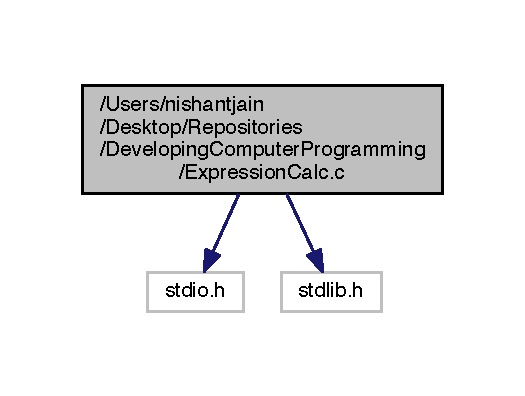
\includegraphics[width=236pt]{_expression_calc_8c__incl}
\end{center}
\end{figure}
\subsection*{Functions}
\begin{DoxyCompactItemize}
\item 
int \hyperlink{_expression_calc_8c_ae66f6b31b5ad750f1fe042a706a4e3d4}{main} ()
\end{DoxyCompactItemize}


\subsection{Function Documentation}
\hypertarget{_expression_calc_8c_ae66f6b31b5ad750f1fe042a706a4e3d4}{\index{Expression\+Calc.\+c@{Expression\+Calc.\+c}!main@{main}}
\index{main@{main}!Expression\+Calc.\+c@{Expression\+Calc.\+c}}
\subsubsection[{main}]{\setlength{\rightskip}{0pt plus 5cm}int main (
\begin{DoxyParamCaption}
{}
\end{DoxyParamCaption}
)}}\label{_expression_calc_8c_ae66f6b31b5ad750f1fe042a706a4e3d4}


Definition at line 4 of file Expression\+Calc.\+c.


\hypertarget{_expression_calc_8c_source}{\section{/\+Users/nishantjain/\+Desktop/\+Repositories/\+Developing\+Computer\+Programming/\+Expression\+Calc.c}
}

\begin{DoxyCode}
00001 \textcolor{preprocessor}{#include <stdio.h>}
00002 \textcolor{preprocessor}{#include <stdlib.h>}
00003 
00004 \textcolor{keywordtype}{void} \hyperlink{_expression_calc_8c_a79cd2ba7236d8017474e3340e169f888}{Extra}();
00005 \textcolor{keywordtype}{void} \hyperlink{_expression_calc_8c_a1f044085ede204d3d2ba2e4db44e7e5d}{CalcFib}(\textcolor{keywordtype}{int} r);                                             \textcolor{comment}{//Function prototype to calculate
       Fibonacci series}
00006 
\hypertarget{_expression_calc_8c_source_l00007}{}\hyperlink{_expression_calc_8c_ae66f6b31b5ad750f1fe042a706a4e3d4}{00007} \textcolor{keywordtype}{int} \hyperlink{_expression_calc_8c_ae66f6b31b5ad750f1fe042a706a4e3d4}{main}()
00008 \{
00009   printf(\textcolor{stringliteral}{"Welcome to Calculator. \(\backslash\)n"});                          \textcolor{comment}{//Welcome Screen}
00010   \textcolor{keywordtype}{char} check;
00011   \textcolor{keywordtype}{int} r;
00012   FILE * Log;
00013   Log = fopen (\textcolor{stringliteral}{"Log.txt"}, \textcolor{stringliteral}{"w+"});                            \textcolor{comment}{//Opening a new file for Logging info. Opening
       in reading and writing mode}
00014       
00015     \textcolor{keywordflow}{do}
00016     \{                                                           
00017       printf(\textcolor{stringliteral}{"Please select an Arithmetic operation from the following: \(\backslash\)n"});           
00018       printf(\textcolor{stringliteral}{"1)Addition \(\backslash\)t 2)Subtraction \(\backslash\)t 3)Multiplication \(\backslash\)t 4)Division \(\backslash\)t 5)Extra Features \(\backslash\)n "});
00019       \textcolor{keywordtype}{int} ch;
00020       \textcolor{keywordtype}{char} opt;
00021       \textcolor{keywordtype}{float} var1, var2;
00022       \textcolor{keywordtype}{float} res;
00023       
00024       scanf(\textcolor{stringliteral}{" %d"}, &ch);                                            \textcolor{comment}{//Input of operation, A SPACE before %d
       makes scanf ignore whitespace}
00025       
00026       \textcolor{keywordflow}{if}(ch!=5)
00027       \{
00028         printf(\textcolor{stringliteral}{"Do you want to use the previous result as one of the operands (Y/N)? \(\backslash\)n"});
00029         scanf(\textcolor{stringliteral}{" %c"}, &opt);                                                 \textcolor{comment}{//Asking user if he wants to
       use saved previous result}
00030       
00031         printf(\textcolor{stringliteral}{"Enter any values for operand(s): \(\backslash\)n"});
00032         \textcolor{keywordflow}{if}(opt==\textcolor{charliteral}{'Y'} || opt==\textcolor{charliteral}{'y'})
00033           \{
00034             printf(\textcolor{stringliteral}{"Operand 1 is the previous result: "});
00035             rewind(Log);
00036             fscanf(Log, \textcolor{stringliteral}{" %f"}, &var1);                                  \textcolor{comment}{//Taking value from the LOG text
       file for variable 1}
00037             printf(\textcolor{stringliteral}{"%f \(\backslash\)n"}, var1);
00038           \}  
00039       
00040         \textcolor{keywordflow}{else} 
00041         \{
00042           printf(\textcolor{stringliteral}{"Operand 1: "}); 
00043           scanf(\textcolor{stringliteral}{"%f"}, &var1);                                       \textcolor{comment}{//Input of variable1}
00044         \}
00045         
00046         printf(\textcolor{stringliteral}{"Operand 2: "}); 
00047         scanf(\textcolor{stringliteral}{" %f"}, &var2);                                    \textcolor{comment}{//This is an optional starting asterisk
       indicates }
00048                                                                 \textcolor{comment}{//that the data is to be read from the
       stream but }
00049                                                                 \textcolor{comment}{//ignored, i.e. it is not stored in the
       corresponding argument. }
00050                                                                 \textcolor{comment}{//Input of variable2}
00051         \textcolor{keywordflow}{switch}(ch)                                              \textcolor{comment}{//Switch case construct: Statements for
       different conditions}
00052         \{
00053           \textcolor{keywordflow}{case} 1: res=var1+var2; \textcolor{keywordflow}{break};
00054           \textcolor{keywordflow}{case} 2: res=var1-var2; \textcolor{keywordflow}{break};
00055           \textcolor{keywordflow}{case} 3: res=var1*var2; \textcolor{keywordflow}{break};
00056           \textcolor{keywordflow}{case} 4: res=var1/var2; \textcolor{keywordflow}{break};
00057         \}
00058          
00059         
00060         printf(\textcolor{stringliteral}{"\(\backslash\)nThe Result= %f \(\backslash\)n"}, res);                         \textcolor{comment}{//Displaying result from file}
00061       
00062         rewind(Log);
00063         fprintf(Log, \textcolor{stringliteral}{" %f"}, res);                               \textcolor{comment}{//Logging the result}
00064       
00065       \}
00066       
00067       \textcolor{keywordflow}{else} \hyperlink{_expression_calc_8c_a79cd2ba7236d8017474e3340e169f888}{Extra}();                                     \textcolor{comment}{//Calling the CalcFib() function and passing
       range as parameter.}
00068       
00069       printf(\textcolor{stringliteral}{"Continue y/n?  "});                                \textcolor{comment}{//Asking user to continue or exit}
00070       scanf(\textcolor{stringliteral}{" %c"},&check);                                      \textcolor{comment}{//A SPACE before %d makes scanf ignore
       whitespace}
00071       
00072     \}\textcolor{keywordflow}{while}(check!=\textcolor{charliteral}{'n'});                 
00073    
00074     fclose(Log);                                                    \textcolor{comment}{// Closing opened text file}
00075    
00076 \textcolor{keywordflow}{return}(0);
00077 \}
00078 
\hypertarget{_expression_calc_8c_source_l00079}{}\hyperlink{_expression_calc_8c_a79cd2ba7236d8017474e3340e169f888}{00079} \textcolor{keywordtype}{void} \hyperlink{_expression_calc_8c_a79cd2ba7236d8017474e3340e169f888}{Extra}()                                               
00080 \{ 
00081   \textcolor{keywordtype}{int} ch,r;
00082   printf(\textcolor{stringliteral}{"\(\backslash\)nSelect from the following options: \(\backslash\)n1)Fibonacci Series \(\backslash\)n"});
00083   scanf(\textcolor{stringliteral}{" %d"},&ch);
00084   \textcolor{keywordflow}{switch}(ch)
00085   \{
00086     \textcolor{keywordflow}{case} 1: printf(\textcolor{stringliteral}{"Enter the range of Fibonacci series: \(\backslash\)n "}); scanf(\textcolor{stringliteral}{" %d"},&r); 
      \hyperlink{_expression_calc_8c_a1f044085ede204d3d2ba2e4db44e7e5d}{CalcFib}(r); \textcolor{keywordflow}{break};
00087   \}
00088 \}
00089 
\hypertarget{_expression_calc_8c_source_l00090}{}\hyperlink{_expression_calc_8c_a1f044085ede204d3d2ba2e4db44e7e5d}{00090} \textcolor{keywordtype}{void} \hyperlink{_expression_calc_8c_a1f044085ede204d3d2ba2e4db44e7e5d}{CalcFib}(\textcolor{keywordtype}{int} r)                                          
00091 \{
00092   \textcolor{keywordtype}{int} j=0, k=1, res;
00093   printf(\textcolor{stringliteral}{"FIBONACCI SERIES: "});
00094   printf(\textcolor{stringliteral}{"%d %d"},j,k); \textcolor{comment}{//printing firts two values.}
00095 
00096     \textcolor{keywordflow}{for}(\textcolor{keywordtype}{int} i=2;i<r;i++)
00097     \{
00098       res=j+k;
00099       j=k;
00100       k=res; 
00101       printf(\textcolor{stringliteral}{" %d"},k);
00102     \}  
00103   printf(\textcolor{stringliteral}{"\(\backslash\)n"}); 
00104 \}
00105 
00106 \textcolor{comment}{// \(\backslash\)image FlowchartCalc.png}
00107 
00108 
\end{DoxyCode}

\hypertarget{_r_e_a_d_m_e_8md}{\section{R\+E\+A\+D\+M\+E.\+md File Reference}
\label{_r_e_a_d_m_e_8md}\index{R\+E\+A\+D\+M\+E.\+md@{R\+E\+A\+D\+M\+E.\+md}}
}

\hypertarget{_r_e_a_d_m_e_8md_source}{\section{/\+Users/nishantjain/\+Desktop/\+Repositories/\+Developing\+Computer\+Programming/\+R\+E\+A\+D\+M\+E.md}
}

\begin{DoxyCode}
00001 Developing-Computer-Programming-Program-Elements-Structure
00002 ==========================================================
00003 
00004 Developing Computer Programming: Program Elements &amp; Structure, challenges, programs and
       documentation
\end{DoxyCode}

%--- End generated contents ---

% Index
\newpage
\phantomsection
\addcontentsline{toc}{chapter}{Index}
\printindex

\end{document}
